\documentclass[a4paper]{article}

\usepackage[english]{babel}
\usepackage[utf8]{inputenc}
\usepackage[T1]{fontenc}
\usepackage{amsmath}
\usepackage{amssymb}
\usepackage{graphicx}
\usepackage[head=26pt, a4paper, margin=1.2in, top=1.2in, bottom=1.2in]{geometry}
\usepackage{eurosym}
\usepackage{listings}
\usepackage{parskip}
\usepackage{float}
\usepackage{listings}
\usepackage{color}
\usepackage{caption}
\usepackage{fancyhdr}
\usepackage{lastpage}
\usepackage{multicol}
\usepackage[hidelinks]{hyperref}


% \DeclareCaptionFont{white}{ \color{white} }
\DeclareCaptionFont{black}{ \color{black} }

\DeclareCaptionFormat{listing}{
  \centering{#1#2#3}
}

\captionsetup[lstlisting]{ format=listing, labelfont=black, textfont=black, singlelinecheck=false, margin=0pt }

\definecolor{mygreen}{rgb}{0,0.6,0}
\definecolor{mygray}{rgb}{0.5,0.5,0.5}
\definecolor{mymauve}{rgb}{0.58,0,0.82}

\lstset{ %
  backgroundcolor=\color{white},   % choose the background color; you must add \usepackage{color} or \usepackage{xcolor}
  basicstyle=\footnotesize,        % the size of the fonts that are used for the code
  breakatwhitespace=false,         % sets if automatic breaks should only happen at whitespace
  breaklines=true,                 % sets automatic line breaking
  captionpos=b,                    % sets the caption-position to bottom
  commentstyle=\color{mygreen},    % comment style
  deletekeywords={...},            % if you want to delete keywords from the given language
  escapeinside={\%*}{*)},          % if you want to add LaTeX within your code
  extendedchars=true,              % lets you use non-ASCII characters; for 8-bits encodings only, does not work with UTF-8
  frame=single,                    % adds a frame around the code
  keepspaces=true,                 % keeps spaces in text, useful for keeping indentation of code (possibly needs columns=flexible)
  keywordstyle=\color{blue},       % keyword style
  language=Matlab,                 % the language of the code
  otherkeywords={*,...},           % if you want to add more keywords to the set
  numbers=left,                    % where to put the line-numbers; possible values are (none, left, right)
  numbersep=5pt,                   % how far the line-numbers are from the code
  numberstyle=\tiny\color{mygray}, % the style that is used for the line-numbers
  rulecolor=\color{black},         % if not set, the frame-color may be changed on line-breaks within not-black text (e.g. comments (green here))
  showspaces=false,                % show spaces everywhere adding particular underscores; it overrides 'showstringspaces'
  showstringspaces=false,          % underline spaces within strings only
  showtabs=false,                  % show tabs within strings adding particular underscores
  firstnumber=2,
  stepnumber=2,                    % the step between two line-numbers. If it's 1, each line will be numbered
  stringstyle=\color{mymauve},     % string literal style
  tabsize=2,                       % sets default tabsize to 2 spaces
  title=\lstname                   % show the filename of files included with \lstinputlisting; also try caption instead of title
}


% ---------------- Page and margin/header/footer Setup -----------------
\pagestyle{fancy}
\fancyhf{} % Clears header and footer
\lhead{\bfseries SIP\\Assignment 2}
\rhead{University of Copenhagen\\Computer Science}
\lfoot{Page \thepage\ of \pageref{LastPage}}
\rfoot{Mads Thoudahl\\Michael Maribo}
\renewcommand{\headrulewidth}{0.4pt}
\renewcommand{\footrulewidth}{0.4pt}
% ----------------------------------------------------------------------

\newcommand{\HRule}{\rule{\linewidth}{0.5mm}}


\begin{document}
\begin{titlepage}
\title{\HRule \\[0.4cm]
\textbf{Signal \& Image Processing }\\Assignment 2\\
\HRule \\[0.4cm]}

\author{
\textbf{Mads Christian Thoudahl} - qmh332\\
\textbf{Michael Mariboe} - njp947\\
\textbf{Nikolai Friis Østergaard} - ltm741\\\\
\textit{Computer Science}\\
\textit{University of Copenhagen}
}

\date{\today}
\maketitle
\thispagestyle{empty}
\end{titlepage}

\newpage

\section*{1 - Histogram based processing}

\subsection*{1.1)}
% \textit{``In mathematical terms, what is the cumulative distribution function (CDF) with respect to the probability density function (PDF) from the continuous point of view ? What can you infer about the variations of the CDF in general?''}\\

In mathematical terms, the \textit{Cumulative Density function} (CDF) relation to the \textit{Probability density function} (PDF) from the continuous point of view is the definite integral from negative infinity to each value of the variable of the function wrt. the variable:
\begin{align}
  cdf(x) = \int_{-\infty}^x pdf(x) \quad \text{d}x
\end{align}

In general, we know that no such thing as a negative probability exists, thus $pdf(x) \: \geq \: 0 \quad \forall \: x$.
This means that whatever infitessimally small part of the area under the function will be nonnegative as well.

Integrating nonnegative parts ensures that the slope of the derivative is nonnegative, in other words $cdf(x)$ is non-decreasing.


\vfill
\subsection*{1.2)}
% \textit{``What are the PDF and CDF of a constant image? What is the CDF corresponding to a constant PDF?''}\\

For a constant image, in a discrete setting where $x, c \in \mathbb{N}$ , all pixels contain the same value constant denoted $c$, thus the probability of that specific value is exactly 1, and the rest is 0, as distribution functions are normalized. It will resemble a single spike when plotted (see \autoref{fig:1.2}a), and somewhat resembles the normalized continous 1d gaussian function, where standard deviation $\sigma \rightarrow 0$, and $x=c$.

\begin{align}
pdf(x) &= \begin{cases} 1 & \text{if } x = c \\ 0 & \text{otherwise} \end{cases} &&&
cdf(x) &= \begin{cases} 1 & \text{if } x \geq c \\ 0 & \text{if } x < c \end{cases}
\end{align}

The \textit{cdf} resembles the 'sigma' function, 'centered' at $x=c$. It generally looks like a 'ski-hill' or a tilted, stretched 'S', but in the constant image it is is a function which increases from zero to one in one step at $x=c$ (\autoref{fig:1.2}b).

The CDF corresponding to a constant PDF (\autoref{fig:1.2}c) is a linear function which increases from zero to one between the minimum and maximum values of the function variable (\autoref{fig:1.2}d).

\begin{figure}[h!]
  \centering
  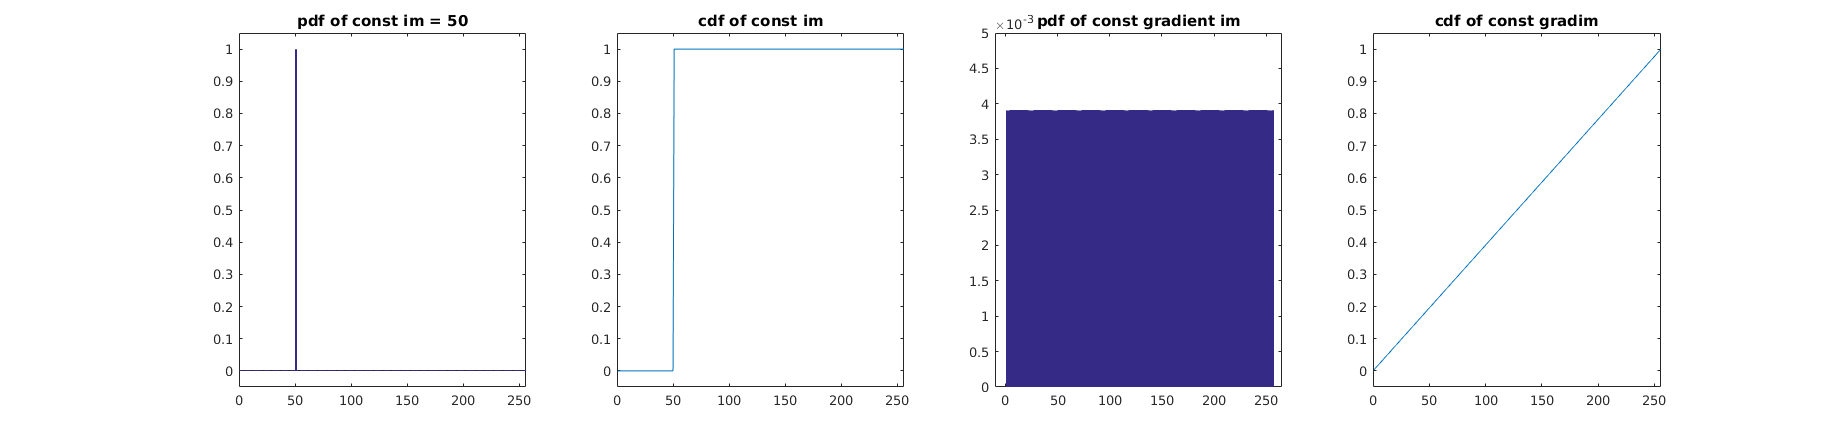
\includegraphics[width=\linewidth]{./1_2a.png}
  \caption{Normalized PDF and CFD in constant / constant gradient greyscale image}
  \label{fig:1.2}
\end{figure}

\newpage
\subsection*{1.3)}
% \textit{``In the discrete setting, implement a MATLAB function that, to a given histogram of a grayscale image, computes its cumulative histogram (you may use MATLAB’s cumsum function and normalize the expression). Display it for the image pout.tif. What do the regions of fast increase of the function correspond to? And what about its flat regions?''}\\

The regions of fast increase of the function corresponds to high counts of pixel intensities and the flat regions corresponds to low counts (or no counts) of pixel intensities.

\begin{figure}[h]
  \centering
  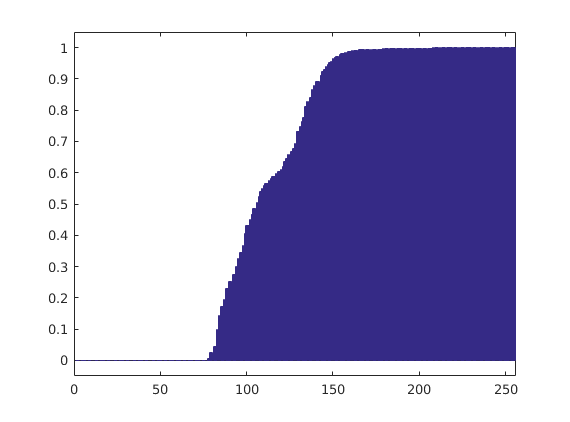
\includegraphics[width=\linewidth]{./1_3.png}
  \caption{Normalized Cumulative Histogram (cdf(h))}
  \label{fig:1.3}
\end{figure}

\begin{figure}[h!]
  \begin{lstlisting}[caption='Code to display Cumulative Histogram']
function [ cs ] = cdf(pdf)
  % pdf is a histogram
  c = double(cumsum(pdf));
  cs = c / c(end);
end

function cs = cumhist(fname)
  I = imread(fname);  % load image
  h = imhist(I);      % get histogram
  ncs = cdf(h);       % calculate 'normalized cumulative sum'
  % display the resulting array
  bar(ncs); axis([0 256 -0.05 1.05]);
end\end{lstlisting}
\end{figure}

\newpage
\subsection*{1.4)}
% \textit{``Given an image I and its CDF C, write a matlab routine that computes the floating-point image C(I) such that the intensity at each pixel (i, j) is C(I(i, j))''}\\

The tricky part here is really to remember that images are stored laid out row-major in matlab, this means that our perception of I(x,y) has to be queried like I(y,x) in matlab.

Running the code will open a figure, that may be queried multiple times, answer will be stated in the title.
The result of the calculation has same effect as asking 'how big a part of the pixels are darker than the one selected?'
This means when pressing a relative dark pixel in the image, the result is low (near $0.0$), and when pressing a relatively bright pixel, the result will be high (near $1.0$).

\vfill
\begin{figure}[h!]
  \centering
  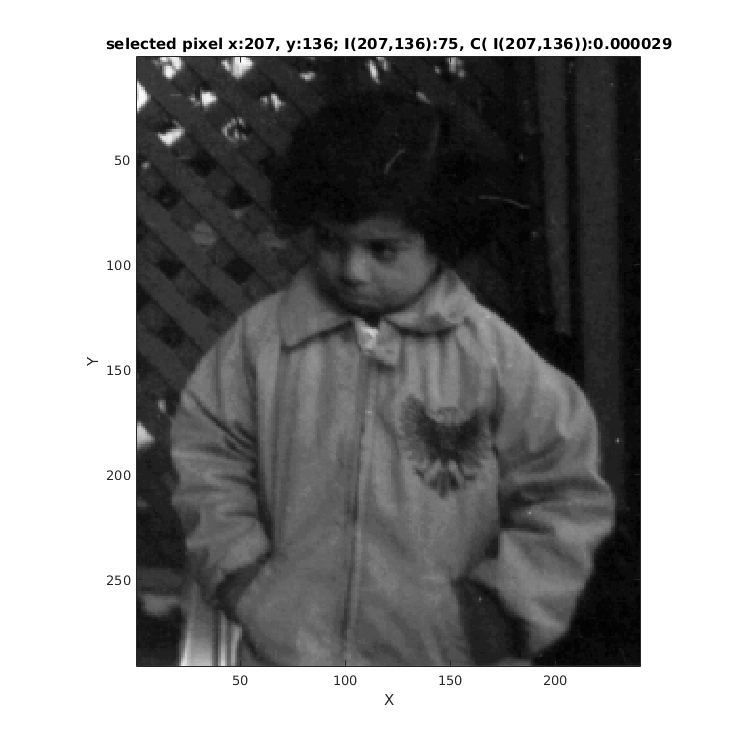
\includegraphics[width=0.45\linewidth, trim={40 40 40 30 }, clip=true]{./1_4a.png}
  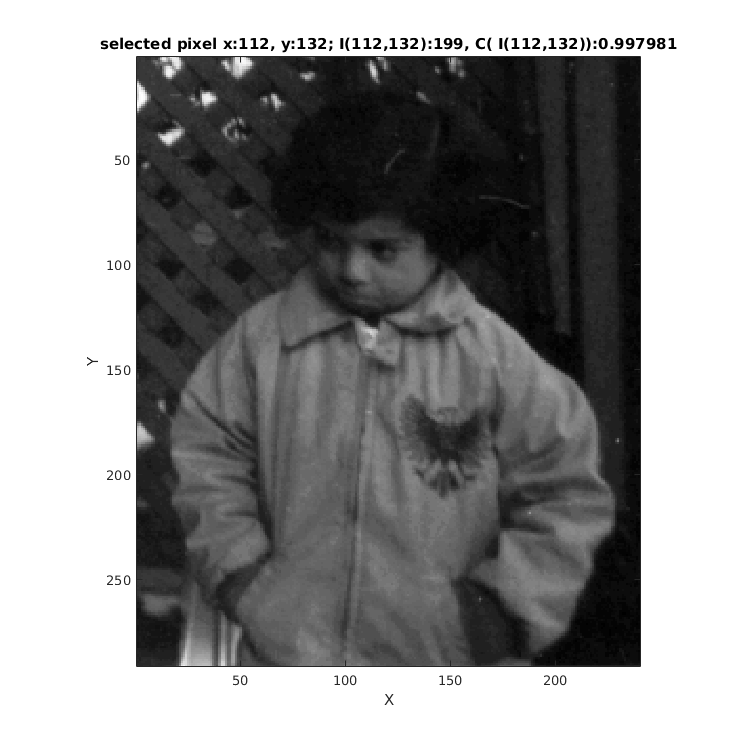
\includegraphics[width=0.45\linewidth, trim={40 40 40 30 }, clip=true]{./1_4b.png}
  \caption{Select a pixel, display intensity and part this pixel is brighter than}
  \label{fig:1.4}
\end{figure}

\vfill
\begin{figure}[h!]
  \begin{lstlisting}[caption='Code to display Cumulative Histogram']
function brighterthan(fname)
  I = imread(fname); h = imhist(I); ncs = cdf(h);
  fmt = 'selected pixel x:%d, y:%d; I(%d,%d):%d, C( I(%d,%d)):%f';
  hFig = figure(1); set(hFig, 'Position', [20 20 750 750]);
  imagesc(I); axis image; colormap(gray); xlabel('X'); ylabel('Y');
  while true
    [x,y] = ginput(1);
    x = round(x); y = round(y);
    s = sprintf(fmt,x,y,x,y,round(I(y,x)),x,y,ncs(I(y,x)))
    title(s);
end\end{lstlisting}
\end{figure}

\newpage
\subsection*{1.5)}
% \textit{``Is the CDF invertible in general and why? To overcome the problem of non-invertibility for histogram matching (cf 3.4.5), we can consider instead a pseudo-inverse. For any CDF function f defined on the integer set {0, .., 255}, we define its pseudo-inverse $f^{-1}$ as follows : $f^{-1} (l) = min{s | f (s) \geq l}$,  where $l \in [0, 1]$. Write and add in your report a MATLAB routine that computes the pseudo-inverse of any given CDF (you may use MATLAB find and min functions)''}

The CDF is not invertible in general, because the inverse isn't a function. Take the example from \autoref{fig:1.3}, because it has a vertical line, it cannot pass the vertical line test. Also, one can see that as no values below the constant exist, $cdf(v)=0$, for $0<v<c$ and $cdf^{-1}(v) = \frac{1}{0}$ and division by zero is an illegal operation.

The pseudo inverse proposed in the assignment text is implemented as follows:
\begin{figure}[h!]
  \begin{lstlisting}[caption='cdf pseudo-inverse implementation']
function [ pseudo_inverse ] = cdfpinv( cdf, l )
  % find the cdf values larger than l, and return the least of them
  pseudo_inverse = min( find(cdf >= l) );
end\end{lstlisting}
\end{figure}

\subsection*{1.6)}
% \textit{``Based on equation (3.25) and on the two previous questions, implement your own MATLAB procedure to perform histogram matching between two images and show results. Plot and compare the cumulative histograms of the original image, the target and the one obtained by histogram matching.''}\\

The \textit{histmatch} procedure is implemented in matlab, and the results are shown in \autoref{fig:1.6} and \autoref{fig:1.7}.


\begin{figure}[h!]
  \centering
  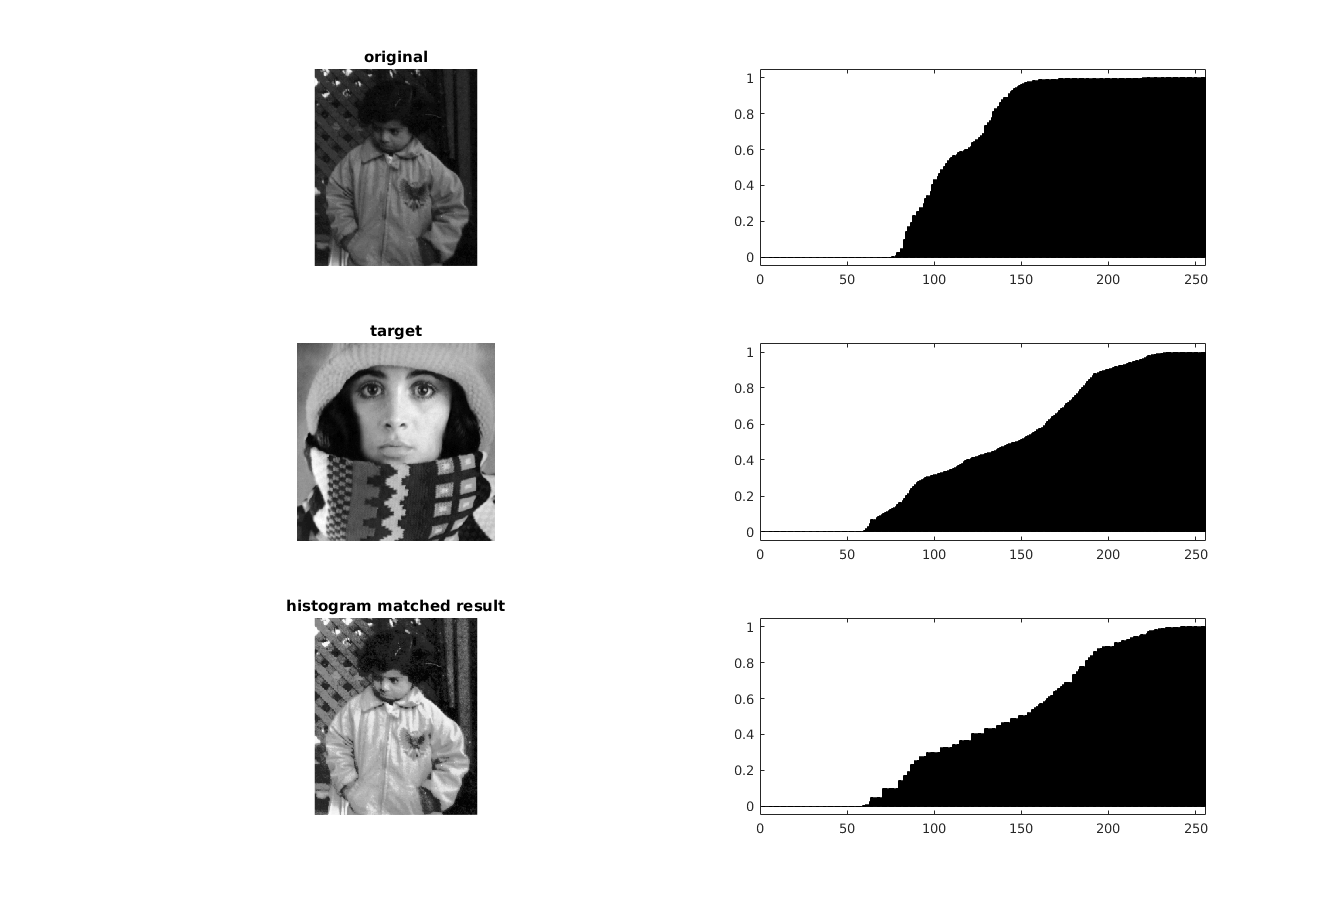
\includegraphics[width=0.6\linewidth, trim={50 30 50 30 }, clip=true]{./1_6.png}
  \caption{Image 'pout.tif' matched with the histogram characteristics of the 'trui.png' image}
  \label{fig:1.6}
\end{figure}

\begin{figure}[h!]
  \begin{lstlisting}[caption='cdf histmatch implementation']
function [ Ix_matched_to_Iz ] = histmatch(I_x, I_z)
  Cx = cdf(pdf(I_x));
  Cz = cdf(pdf(I_z));
  Czinv = uint8(pinv( Cz, Cx ));
  Ix_matched_to_Iz = applymapping(I_x, Czinv);
end
im        = imrea\tilde{I}_1d('images/pout.tif');
targetim  = imread('images/trui.png');
matched   = histmatch(im, targetim);\end{lstlisting}
\end{figure}



\newpage
\subsection*{1.7)}
% \textit{``Apply it in the particular case where the target cumulative histogram is the one corresponding to a constant histogram. Compare the result to MATLAB histeq built-in function.''}\\

The histmatch function applied to the \texttt{pout.tif} image and the constant histogram. It seems that the effect is equal to the matlab \textit{histeq} build-in function.

\begin{figure}[h!]
  \centering
  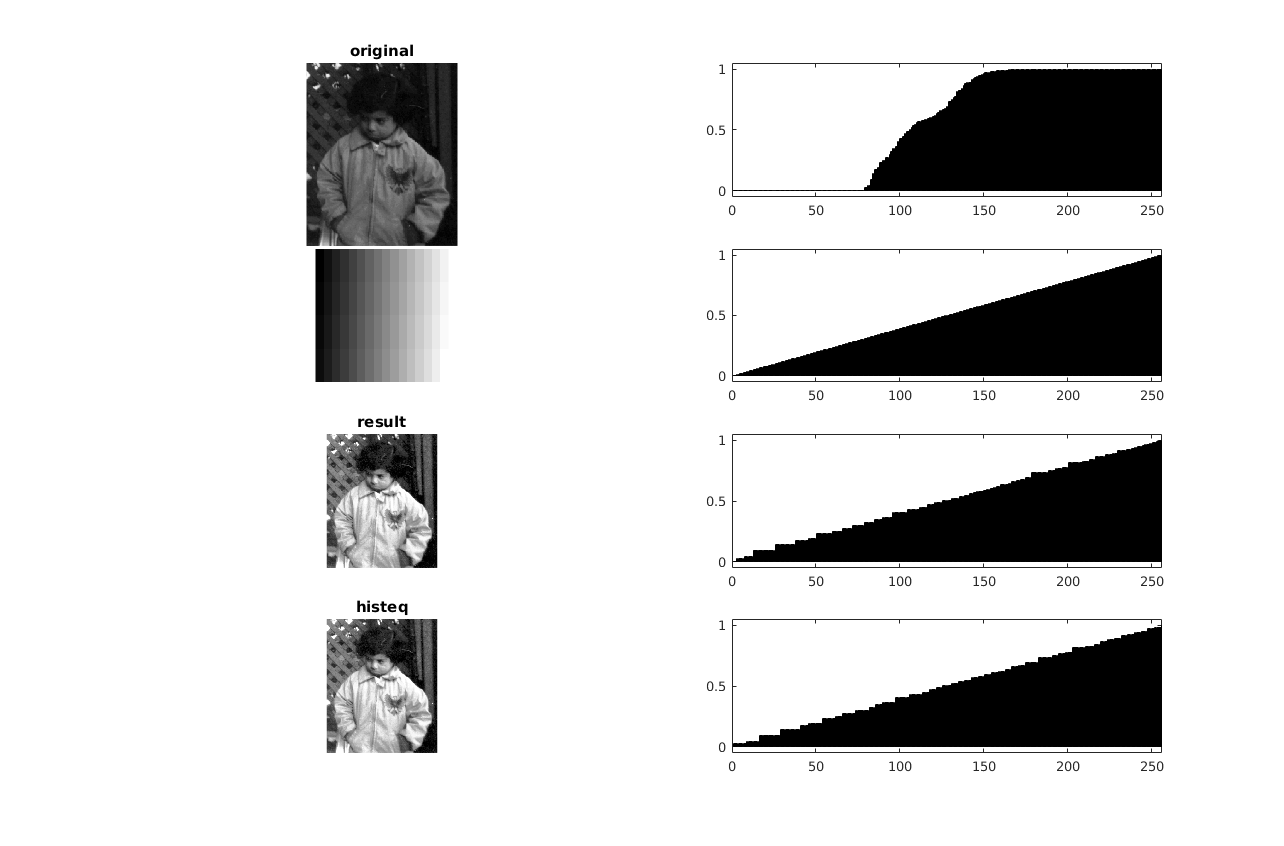
\includegraphics[width=0.8\linewidth, trim={40 40 40 30 }, clip=true]{./1_7.png}
  \caption{Image 'pout.tif' matched with uniform pdf image, and compared to matlab histeq}
  \label{fig:1.7}
\end{figure}

\begin{figure}[h!]
  \begin{lstlisting}[caption='application of histmatch to constant histogram image']
im        = imread('images/pout.tif');
targetim  = reshape(uint8(0:255),16,16);  % constant gradient (histogram)
matched   = histmatch(im, targetim);
he        = histeq(im);

plots...\end{lstlisting}
\end{figure}

\newpage
\subsection*{1.8)}
% \textit{``Let I 1 and I 2 be two images with cumulative histograms C 1 and C 2 . Let’s introduce : $\phi = \frac{1}{2} \left( C_1^{(-1)} + C_2^{(-1)} \right) $ and the images $\tilde{I}1 = \phi(C1 (I1))$ and $\tilde{I}2 = \phi(C2 (I2 )) $ called the midway specifications of I1 and I2. If I1 and I2 are two constant images with respective values a and b, prove that the midway specifications are both equal to the constant image (a+b)/2? Is the cumulative histogram of the midway specifications equal to the average of the cumulative histograms ? ''}\\

\subsection*{1}
Remeber definition on pseudo inverse: $C^{-1}(l) = min \{ \left. s \right|_{C(s) \geq l} \}$ for $s \in \{0,..,255\}$
\begin{align}
  \tilde{I}_1 &= \phi(C_1(I_1)) &&&  \tilde{I}_2 &= \phi(C_2(I_2))\\
  \tilde{I}_1 &= \frac{1}{2} \left( C_1^{(-1)}(C_1(a)) + C_2^{(-1)}(C_1(a)) \right) &&&
  \tilde{I}_2 &= \frac{1}{2} \left( C_1^{(-1)}(C_2(b)) + C_2^{(-1)}(C_2(b)) \right)\\
  \tilde{I}_1 &= \frac{1}{2} \left( a + \begin{cases}
                              0 & \text{if } a < b \\
                              b & \text{if } b \leq a
                            \end{cases} \right) &&&
  \tilde{I}_2 &= \frac{1}{2} \left( \begin{cases}
                          0 & \text{if } b < a \\
                          a & \text{if } a \leq b
                        \end{cases} + b \right) \\
  \tilde{I}_1 &= \begin{cases}
      \frac{a}{2} & \text{if } a < b \\
      \frac{a+b}{2} & \text{if } b \leq a
                 \end{cases} &&&
  \tilde{I}_2 &= \begin{cases}
      \frac{b}{2} & \text{if } b < a \\
      \frac{a+b}{2} & \text{if } a \leq b
                 \end{cases}
\end{align}

It seems I have somehow failed to prove Imagethat $\tilde{I}_1 = \tilde{I}_2$ even if the images $I_1$ and $I_2$ are constant.

\subsection*{2}
\begin{figure}[h!]
  \centering
  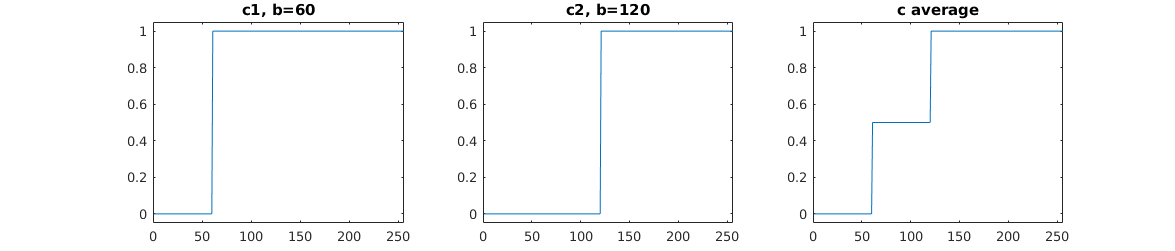
\includegraphics[width=\linewidth, trim={10 0 0 0 }, clip=true]{./1_8.png}
  \caption{Images with averaged cumulative histograms}
  \label{fig:1.8}
\end{figure}

Assuminapplication of histmatch to constant histogramg that $\tilde{I}_1 = \tilde{I}_2$, \autoref{fig:1.8} shows that the cumulative histogram of the midway specifications cannot be equal to the average of the cumulative histograms. The reason is that there is clearly 2 'jumps' on the average cdf, and there would be only one jump if $\tilde{I}_1 = \tilde{I}_2$.

\newpage
\subsection*{1.9)}
% \textit{``Write a MATLAB function that computes the midway specifications of two images. Show the result on the images movie.flicker1.tif and movie.flicker2.tif located in the Test Images folder (convert them to grayscale) which corresponds  to two successive frames of the 1948 movie "Les aventures des Pieds-Nickeles" (copyright Marc Sandberg). How would you generalize midway equalization to an arbitrary number of images ?''}\\

\autoref{fig:1.9ab} shows the two original images in the top row, and it is seen that the leftmost seems darker, which is confirmed by the cdf displayed underneath the image.
In the second row, the two images are 'maidwayed' with respect to the other, and seeming at a similar intensity level on visual inspection, which is confirmed by the cdf's below, which are both very similar, and both looks like a midway compromise of the two top ones.

\begin{figure}[h!]
  \centering
  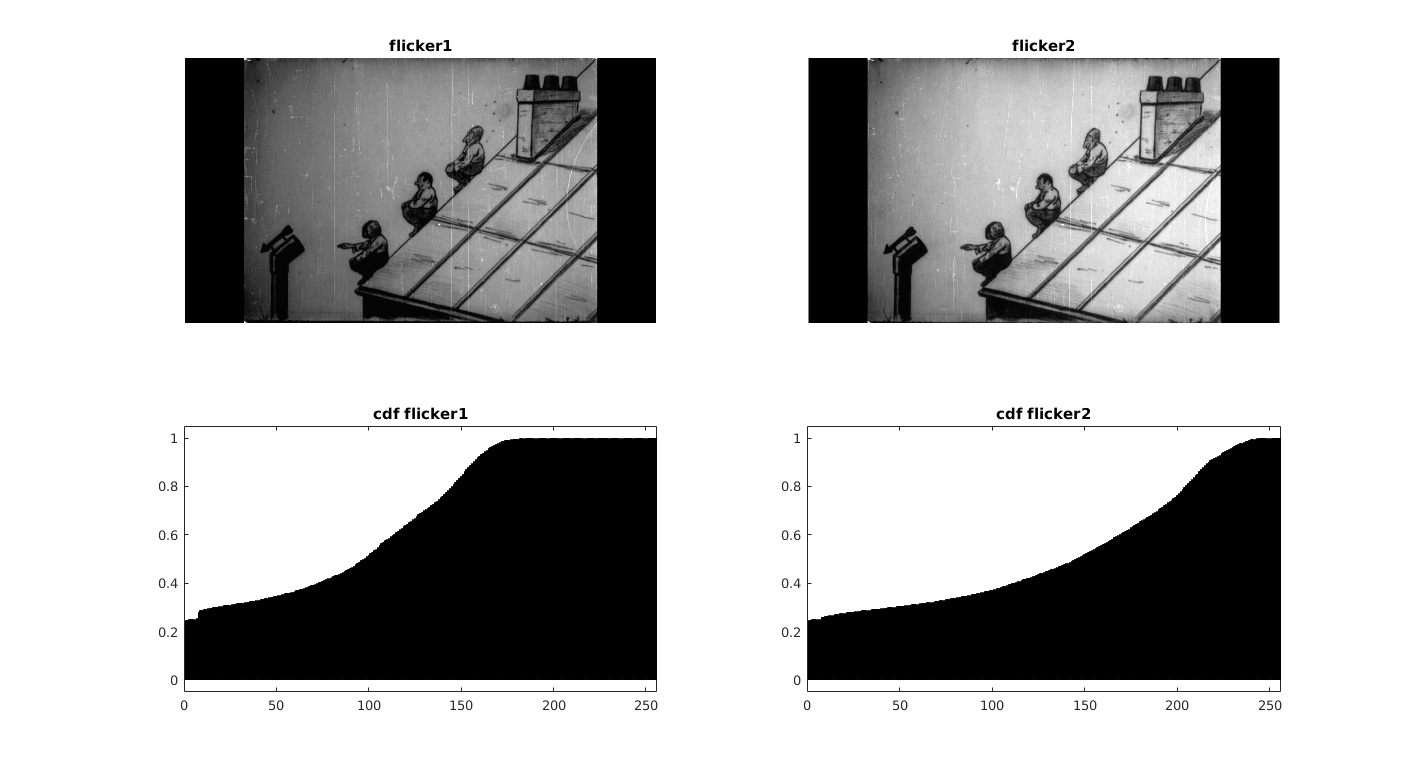
\includegraphics[width=0.8\linewidth, trim={35mm 0mm 35mm 0mm }, clip=true]{./1_9a.png}
  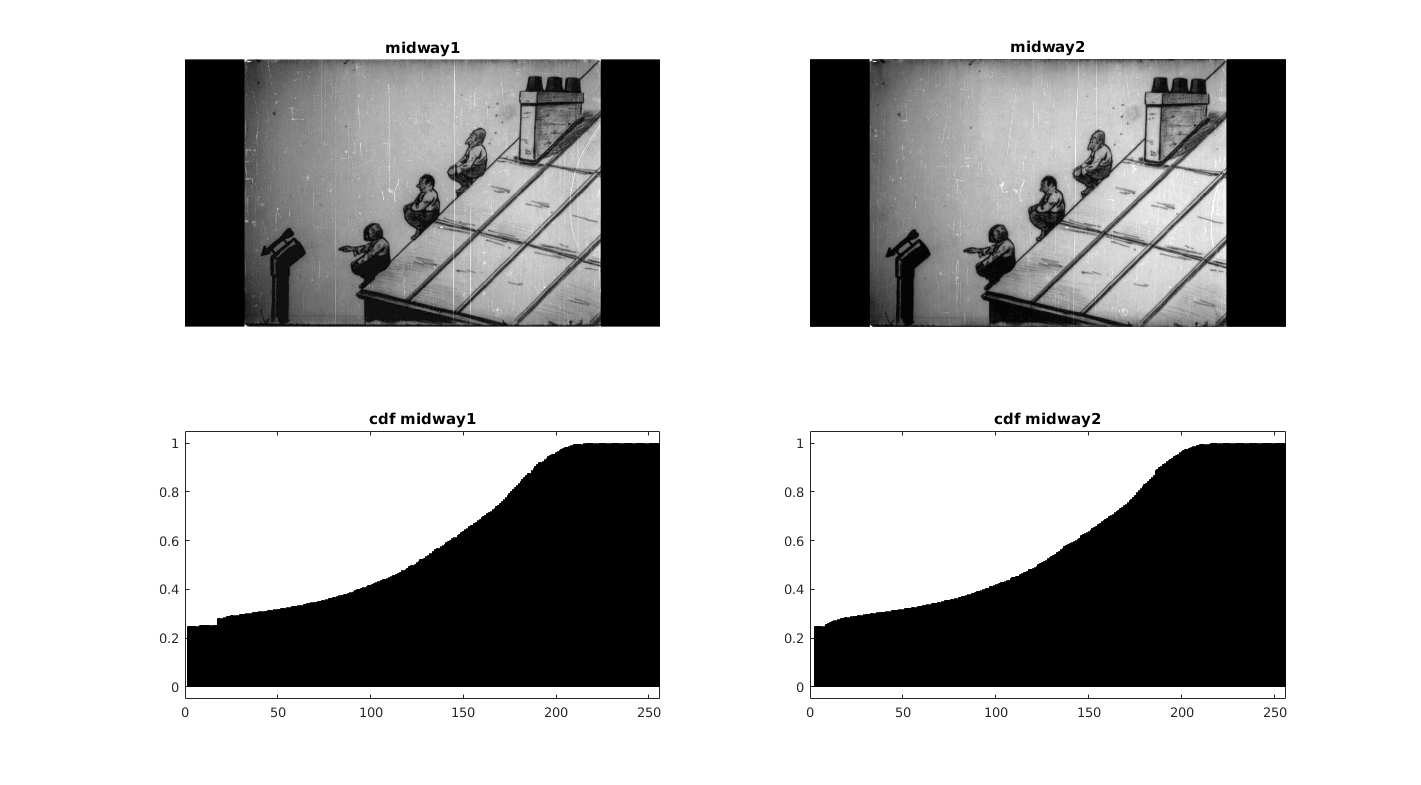
\includegraphics[width=0.8\linewidth, trim={35mm 0mm 35mm 0mm }, clip=true]{./1_9b.png}
  \caption{Original image frames, and midwayed image frames}
  \label{fig:1.9ab}
\end{figure}

\autoref{fig:1.9c} shows the absolute difference in the images, which is of course big along the edges of movement in the two different frames, but further it is evident that the intensity of the original frames differ very much on average, and this difference is almost totally gone in the 'midway'ed' imageset.

\begin{figure}[h!]
  \centering
  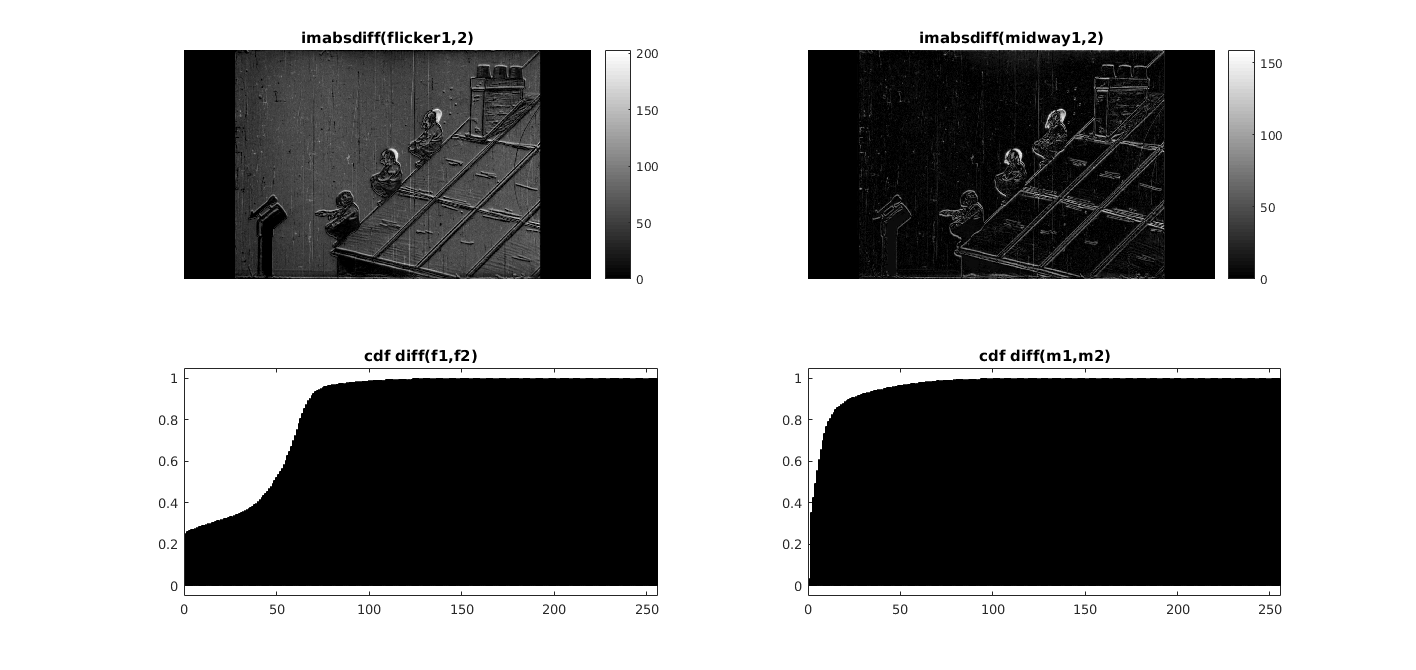
\includegraphics[width=0.8\linewidth, trim={110 0 110 0 }, clip=true]{./1_9c.png}
  \caption{Absolute difference of originals vs midwayed image frames}
  \label{fig:1.9c}
\end{figure}

To generalize the midway equalization, to an arbitrary number $n$ of images, it is written:
$$ \phi = \frac{1}{n} \sum_{i=1}^{n} C^{(-1)}_i $$
The matlab function IS generalized, it currently returns an midway'ed version of the first image argment, 'averaged' with them all.

\begin{figure}[h!]
  \begin{lstlisting}[caption='Midway function and its application.']
function out = midway(Is)
  % general midway function, taking up to n images, usage midway({im_1, .., im_n})
  phi = zeros([1 256]);  n  = length(Is);
  I   = Is{1};           CI = cdf(pdf(I));
  for i=1:n
      C    = cdf(pdf(Is{i}));
      Cinv = pinv(C, CI);
      phi  = phi + Cinv;
  end
  phi = uint8( phi / n );
  out = applymapping(I, phi);
end

im3  = midway({im1, im2});
im4  = midway({im2, im1});

d12 = imabsdiff(im1,im2);
d34 = imabsdiff(im3,im4);\end{lstlisting}
\end{figure}

\clearpage
\section*{2 - Image filtering and enhancements}

\section*{3 - Bonus questions}

\clearpage
\appendix
\section{helper methods}
\begin{figure}[h!]
  \begin{lstlisting}[caption='applies a mapping']
function out = applymapping(in, map)
    % apply the mapping
    [cs rs] = size(in);
    out = uint8(zeros([cs rs]));
    for r = 1:rs
        for c = 1:cs
            out(c,r) = map( in(c,r)+1 );
        end
    end
end\end{lstlisting}
\end{figure}

\end{document}
